\documentclass[border=3pt,varwidth]{standalone}
\usepackage{amsmath,amssymb}
\usepackage{tikz}
\usetikzlibrary{arrows.meta,calc,decorations.markings,patterns,positioning,angles,quotes}
\tikzset{
  >=Stealth,
  every node/.style={font=\normalsize},
  wire/.style={line width=0.9pt},
  thinwire/.style={line width=0.6pt},
  fieldline/.style={line width=0.6pt,-{Stealth[length=2.2mm]}},
  axis/.style={line width=0.7pt,-{Stealth[length=2.2mm]}},
  dashedwire/.style={line width=0.9pt,dash pattern=on 3pt off 2pt},
  resistor/.style={line width=0.9pt},
  chargepos/.style={circle,draw,line width=0.8pt,minimum size=5mm,inner sep=0pt},
  dotcharge/.style={circle,fill,inner sep=0pt,minimum size=2.4pt}
}
% Draw a resistor box centered at (x,y) with width w, height h, horizontal
\newcommand{\resbox}[4]{%
  % #1=x #2=y #3=halfwidth #4=label
  \draw[resistor] (#1-#3,#2-0.18) rectangle (#1+#3,#2+0.18);
  \ifx\\#4\\\else\node[above=2pt] at (#1,#2+0.18) {#4};\fi
}
% Battery symbol: long thin line (+) then short thick line (-), centered at (x,y)
\newcommand{\battery}[2]{%
  % #1=x #2=y ; long line left=+, short line right=- by default orientation
  \draw[wire] (#1-0.09,#2-0.32) -- (#1-0.09,#2+0.32);
  \draw[line width=2.6pt] (#1+0.09,#2-0.16) -- (#1+0.09,#2+0.16);
}

\begin{document}
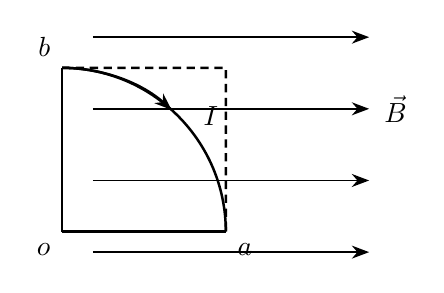
\begin{tikzpicture}[scale=1.3]
  \coordinate (o) at (0,0);
  \coordinate (b) at (0,1.6);
  \coordinate (a) at (1.6,0);
  \draw[wire] (o) -- (b);
  \draw[wire] (o) -- (a);
  \draw[dashedwire] (b) -- (1.6,1.6) -- (a);
  \draw[wire,-{Stealth[length=2.2mm]}] (b) arc[start angle=90,end angle=48,radius=1.6];
  \draw[wire] (b) arc[start angle=90,end angle=0,radius=1.6];
  \node[below left=1pt] at (o) {$o$};
  \node[above left=1pt] at (b) {$b$};
  \node[below right=1pt] at (a) {$a$};
  \node[above right=2pt] at (1.25,0.9) {$I$};
  % uniform field B, horizontal field lines with arrows, to the right
  \foreach \y in {1.9,1.2,0.5,-0.2} {
    \draw[fieldline] (0.3,\y) -- (3.0,\y);
  }
  \node[right=2pt] at (3.0,1.2) {$\vec B$};
\end{tikzpicture}
\end{document}
